% Exercise 3, Burgess et al. (2015) replication with did_multiplegt_dyn.


\noindent \textbf{Given.} A district year panel of all 41 Kenyan districts from 1963 to 2011 (2009 district year observations, balanced). The outcome \texttt{exp\_dens\_share} is the share of national road expenditure received by a district, divided by the district's 1962 population share. The treatment \texttt{president} is a binary indicator equal to one when the district is coethnic with the serving president. The covariates \texttt{pop1962}, \texttt{area}, \texttt{urbrate1962}, \texttt{earnings}, \texttt{wage\_employment}, \texttt{value\_cashcrops} are time invariant 1963 era characteristics.\\

\noindent We are asked to use \texttt{did\_multiplegt\_dyn} to estimate dynamic treatment effects of being coethnic with the serving president on road expenditure. Justify option choices, interpret the event study. Check robustness with Burgess covariates. Investigate whether the same package can estimate the effects of switching out of coethnicity using the method in Web Appendix 1.6 of \citet{dCDH2024}.\\

 \noindent Three presidents serve over the panel: Kenyatta (Kikuyu, 1963 to 1978), Moi (Kalenjin, 1979 to 2002) and Kibaki (Kikuyu, 2003 to 2011). The treatment indicator therefore takes three regime values across 49 calendar years. Reading the data,
\begin{itemize}\setlength\itemsep{0pt}
  \item 28 districts are never coethnic with any president (controls throughout).
  \item 7 districts are coethnic under Kenyatta and Kibaki but not under Moi.
  \item 6 districts are coethnic under Moi but not under Kenyatta or Kibaki.
\end{itemize}
All 13 switching districts therefore experience their first treatment change in 1979 and their second in 2003. There is no variation in first switch dates across the switching subsample. This matters for Part 3 below.\\

\noindent All analysis is run in R. The static two way fixed effects regression is fit with \texttt{fixest}; the dynamic difference in differences estimator is the \texttt{did\_multiplegt\_dyn} function from the \texttt{DIDmultiplegtDYN} package. The full pipeline is in \texttt{analysis.R}.

\paragraph{Sanity check via static TWFE.} Before running \texttt{did\_multiplegt\_dyn} we replicate the static specification of Burgess Table 1 with a two way fixed effects regression. With district and year fixed effects and standard errors clustered by district,
\[
\widehat\beta_{\text{Col 1}} = 0.9746 \; (0.3546), \qquad \widehat\beta_{\text{Col 3}} = 0.9568 \; (0.3464),
\]
where Col 3 adds the six 1963 covariates (demography and economic activity) interacted with a linear time trend. Both numbers match Burgess Table 1 Panel A to two decimals: their Column 1 reports $0.97$ $(0.36)$ and their Column 3 reports $0.96$ $(0.35)$. Column 4 of Burgess Table 1 additionally includes economic geography indicators (corridor, border, distance to Nairobi) that are not in the supplied dataset, so we cannot replicate that column. The sample mean of \texttt{exp\_dens\_share} is $1.25$, so a coefficient near $0.97$ amounts to nearly doubling the average. This is the order of magnitude headline result of \citet{burgess2015}.

\subsection*{Part 1}

\paragraph{Option choices.}
\begin{itemize}\setlength\itemsep{0pt}
  \item \texttt{effects(5)}: report five post switch horizons. The shorter regime, Kibaki 2003 to 2011, has nine years of post switch data; five comfortably fits inside both regimes.
  \item \texttt{placebo(3)}: three pre switch periods, used to test parallel trends and no anticipation.
  \item \texttt{cluster(distnum)}: cluster standard errors at the district level. There are 41 clusters, which is at the lower end of the asymptotic comfort zone but standard for this literature.
  \item No \texttt{trends\_lin} or \texttt{controls} in this baseline. We will add the Burgess controls in Part 2.
\end{itemize}

\paragraph{Estimates.}
\begin{center}
\begin{tabular}{rrrr}
\toprule
Horizon $\ell$ & $\widehat{\mathrm{DID}}_\ell$ & SE & N switchers \\
\midrule
1 & $3.175$ & $2.181$ & 6 \\
2 & $2.853$ & $1.648$ & 6 \\
3 & $2.423$ & $1.395$ & 6 \\
4 & $3.881$ & $1.009$ & 6 \\
5 & $2.739$ & $0.469$ & 6 \\
\midrule
Av\_tot\_effect & $3.014$ & $1.171$ & 30 switch periods \\
\bottomrule
\end{tabular}
\end{center}
The joint test that all five dynamic effects are zero rejects with $p < 0.001$. Average cumulative effect over 30 switch periods is $3.01$ with SE $1.17$, significant at the 5\% level. Placebos at horizons $-1, -2, -3$ are $0.25, 0.04, 0.59$ respectively, each individually insignificant, but the joint placebo test gives $p = 0.045$ which is borderline. The latter is a mild flag against strict parallel trends.\\

 The dynamic effects are all positive and in the same order of magnitude as the static estimate, scaled up because $\mathrm{DID}_\ell$ is the long difference effect over $\ell$ periods rather than a per period effect. The largest point estimate is at $\ell = 4$ and the smallest at $\ell = 3$; the pattern is roughly flat with a peak in the middle, suggesting that the coethnicity premium materialises quickly after a regime change and persists. The event study figure shows the same pattern visually.

\begin{figure}[h]
\centering
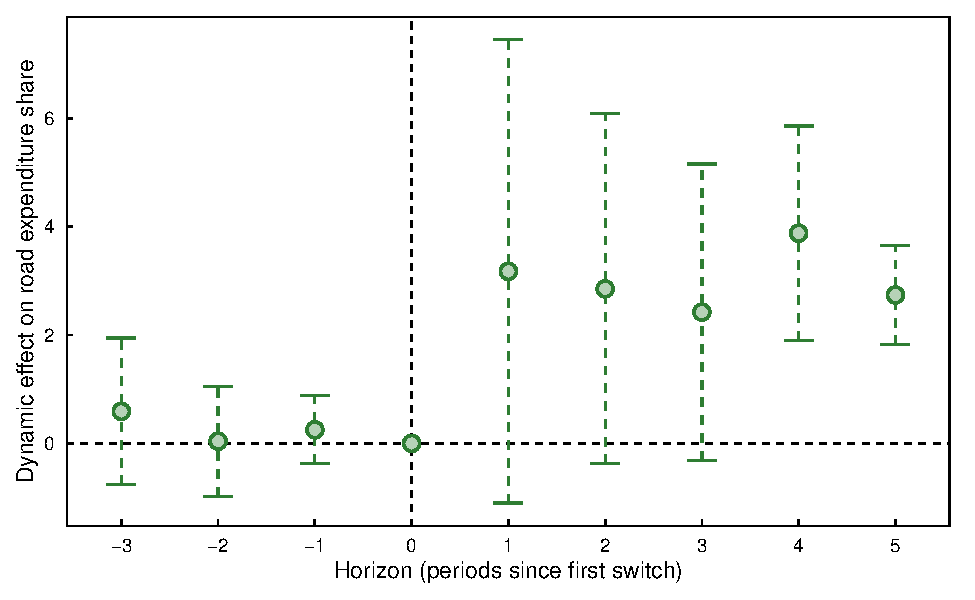
\includegraphics[width=0.75\textwidth]{exercise3/output/ex3_part1_event.pdf}
\caption{Dynamic effects of coethnicity on road expenditure, baseline specification. Horizon zero corresponds to the year of the first switch. Vertical lines are 95 percent confidence intervals based on district level clustered standard errors.}
\label{fig:ex3_part1}
\end{figure}

\subsection*{Part 2}

 The Burgess equation is
\[
\text{road}_{dt} = \gamma_d + \alpha_t + \beta \cdot (\text{coethnic district}_{dt}) + \theta \cdot \bigl(X_{d, 1963} \times (t - 1963)\bigr) + u_{dt}.
\]
Here $X_{d, 1963}$ is a vector of 1963 era district characteristics and $(t - 1963)$ is a calendar year trend. The interaction $X_{d, 1963} \times (t - 1963)$ is constant per district and linear in time, so it is a valid time varying continuous covariate from the perspective of \texttt{did\_multiplegt\_dyn}. Concretely, we construct
\[
\text{var\_tr}_{dt} = \text{var}_{d, 1963} \cdot (t - 1963)
\]
for each of the six covariates and pass them to the \texttt{controls()} option. The Burgess Table 1 sequence Cols 2 to 4 adds demographics first, then economic activity. We do this in two specifications.

\paragraph{Estimates.}
\begin{center}
\begin{tabular}{rrrrrrr}
\toprule
& \multicolumn{2}{c}{Baseline (Part 1)} & \multicolumn{2}{c}{Plus demographics} & \multicolumn{2}{c}{Plus all six} \\
\cmidrule(lr){2-3}\cmidrule(lr){4-5}\cmidrule(lr){6-7}
Horizon $\ell$ & $\widehat{\mathrm{DID}}_\ell$ & SE & $\widehat{\mathrm{DID}}_\ell$ & SE & $\widehat{\mathrm{DID}}_\ell$ & SE \\
\midrule
1 & $3.175$ & $2.181$ & $3.180$ & $2.176$ & $3.181$ & $2.177$ \\
2 & $2.853$ & $1.648$ & $2.863$ & $1.640$ & $2.865$ & $1.640$ \\
3 & $2.423$ & $1.395$ & $2.439$ & $1.380$ & $2.441$ & $1.382$ \\
4 & $3.881$ & $1.009$ & $3.902$ & $0.997$ & $3.905$ & $0.996$ \\
5 & $2.739$ & $0.469$ & $2.765$ & $0.465$ & $2.769$ & $0.463$ \\
\midrule
Av\_tot\_effect & $3.014$ & $1.171$ & $3.030$ & $1.157$ & $3.032$ & $1.158$ \\
\bottomrule
\end{tabular}
\end{center}

Adding Burgess covariates leaves point estimates essentially unchanged. Average cumulative effects move from $3.014$ to $3.030$ to $3.032$ across the three columns. Standard errors fall slightly with each additional control. The joint null on dynamic effects is rejected with $p < 0.001$ in all three specifications. The joint placebo $p$ values are $0.045$, $0.048$ and $0.049$ respectively, all borderline rather than firmly rejected.\\

The Burgess covariates therefore can be implemented in \texttt{did\_multiplegt\_dyn}, with one important caveat about interpretation. The \texttt{controls()} option accepts time varying continuous covariates and uses them to relax the parallel trends assumption: it allows the outcome trend to depend linearly on the controls. The Burgess $X_{d, 1963} \times (t - 1963)$ interactions are time varying continuous (constant per district, linear in time), so they qualify mechanically and the package runs without complaint. The interpretation is not identical to Burgess's static two way fixed effects with controls. The \citet{dCDH2024} estimator targets dynamic average treatment effects on switchers, while Burgess targets a static average effect on the treated. But the robustness exercise is in the same spirit and gives the same substantive conclusion: the dynamic estimates do not move when 1963 demographics or economic activity, interacted with the linear trend, are added. Two further notes worth keeping in mind. First, the package will not accept dummy variables in \texttt{controls()}; categorical controls have to go through the \texttt{trends\_nonparam} option instead. Our covariates are all continuous, so this limitation does not bind here. Second, with only six controls and 41 districts the asymptotic theory is being pushed.

\subsection*{Part 3}

 Web Appendix 1.6 of \citet{dCDH2024} works inside a restricted treatment structure called Design 2: $D_{g,t} = \mathbf{1}\{E_g \ge t \ge F_g\}$, where $F_g$ is the period a unit first switches into treatment and $E_g$ is the period it switches out (with $E_g = T + 1$ for units that never leave). Within Design 2 the paper defines two separately identifiable parameters, a switch in effect $\delta^+_\ell$ and a switch out effect $\delta^-_\ell$, the latter being what Question 3 asks about. The appendix's recipe for $\delta^-_\ell$ is to run \texttt{did\_multiplegt\_dyn} on the subsample of $(g, t)$ where group $g$ has already switched into treatment at or before $t$, with the treatment redefined as a $1 \to 0$ indicator and with $F_g$ included in \texttt{trends\_nonparam}. Assumption 16 of the appendix underlies the procedure: the controls must share the same switch in date $F_g$ as the unit whose switch out is being estimated.\\

The 41 Kenyan districts fall into three regime classes. Each column under a president's name shows the value of \texttt{president} during that regime.
\begin{center}
\resizebox{\textwidth}{!}{%
\begin{tabular}{lccccl}
\toprule
 & & Kenyatta & Moi & Kibaki & \\
Class & $n$ & 1963 to 78 & 1979 to 2002 & 2003 to 11 & Design 2 compatible? \\
\midrule
Never coethnic               & 28 & 0 & 0 & 0 & n.a., no switch in date \\
Moi coethnic                 & 6  & 0 & 1 & 0 & yes, $F_g = 1979,\, E_g = 2003$ \\
Kenyatta and Kibaki coethnic & 7  & 1 & 0 & 1 & no, path is not monotone \\
\bottomrule
\end{tabular}%
}
\end{center}

This mapping produces two distinct failure modes for the appendix's procedure. First, the 7 Kikuyu districts do not fit the Design 2 template at all. Design 2 requires a single contiguous block of treatment, $0 \to 1 \to 0$. The Kikuyu districts experience $1 \to 0 \to 1$ across the panel, which is not monotone and falls outside the framework in which $\delta^-_\ell$ is defined.

Second, the 6 Moi districts do fit Design 2, but the procedure still cannot be executed on them. Their switch in date $F_g$ is uniformly 1979 and their switch out date $E_g$ is uniformly 2003. Assumption 16 requires controls with the same $F_g = 1979$ that have not yet switched out by $E_g + \ell$. There are no such controls in the panel, because every Moi coethnic district switches out simultaneously in 2003 and the 7 other Moi era switchers fall outside Design 2.\\

What \texttt{analysis.R} actually runs is a coarse proxy for the appendix recipe: two \texttt{tryCatch} blocks against the package. Route A passes \texttt{switchers = "out"} on the \texttt{president} treatment. Route B recodes $\widetilde D_{dt} = 1 - D_{dt}$ and passes \texttt{switchers = "in"}. Each call is wrapped in \texttt{tryCatch()} so the script runs to completion, and the captured message is printed via \texttt{writeLines()}. Both routes return the same hard error from the R implementation, reproduced verbatim:
\begin{quote}\small\itshape
No treatment effect can be estimated. \\
\hspace*{1em}This is because Design Restriction 1 in de Chaisemartin \& D'Haultfoeuille (2024) is not satisfied in the data, given the options requested. \\
\hspace*{1em}This may be due to the fact that groups' period-one treatment is continuous, or takes a large number of values, and you have not specified the continuous option. \\
\hspace*{1em}If so, you can try to specify this option. \\
\hspace*{1em}If the issue persists even with this option, this means that all groups experience their first treatment change at the same date. \\
\hspace*{1em}In this situation, estimators of de Chaisemartin \& D'Haultfoeuille (2024) cannot be used.
\end{quote}
The error lists two possible causes. The first, a continuous or high cardinality period one treatment, does not apply because \texttt{president} is binary. The second is the one that does apply: every switching district has its first treatment change in 1979, so Design Restriction 1's staggered timing requirement is violated. The same simultaneity breaks Assumption 16 for the full appendix recipe.\\

The conclusion is that the effects of switching out of coethnicity cannot be estimated with \texttt{did\_multiplegt\_dyn} on this dataset. The obstacle is structural: the 7 Kikuyu districts fall outside Design 2 because of their not monotone treatment path, and the 6 Kalenjin districts share $F_g$ and $E_g$ so Assumption 16 has no admissible controls. The procedure in Web Appendix 1.6 would apply if Kenya had had more presidents, or if the coethnic transitions had been staggered across districts.
